\documentclass{article} % article, book, presenation, beamer

\usepackage{geometry} % This package allows the editing of the page layout
\usepackage{amsmath}  % This package allows the use of a large range of mathematical formula, commands, and symbols
\usepackage{graphicx}  % This package allows the importing of images
\usepackage{color}
\usepackage{hyperref}
\hypersetup{colorlinks=true, linkcolor=blue, urlcolor=blue, citecolor=blue}

% \usepackage[a5paper,landscape,height=8cm,top=2.5cm,includehead=true,width=15cm]{geometry}

\newcommand{\question}[2][]{\begin{flushleft}
    \textbf{Question #1}: \textit{#2}
\end{flushleft}}

\newcommand{\sol}{\textbf{Solution}:} %Use if you want a boldface solution line

\newcommand{\maketitletwo}[2][]{\begin{center}
    \Large{\textbf{Assignment #1}
        Course Title} % Name of course here
    \vspace{5pt}
    
    \normalsize{Matthew Frenkel  % Your name here
    
    \today}        % Change to due date if preferred
    \vspace{15pt}
\end{center}}

\begin{document}

\title{this is my first test}
% \subtitle{Feb 2024}
\author{Akbar Baghbani}
\date{\today}
\maketitle

\pagenumbering{roman}
\tableofcontents
\newpage
\pagenumbering{arabic}
\section{first part}
    this is my first text that I write for testing latex, seems it's so easy to use the command in text file.

    \section{second part}
    as second part I want to write some text data just to test.

    \begin{align*}
        \int_0^2 x^2 &= \left. \frac{x^3}{3} \right|_0^2 \\
                     &= \frac{2^3}{3}-\frac{0^3}{3}\\
                     &= \frac{8}{3}
    \end{align*}

    \question[1]{Here is my first question} 
    
    YOUR SOLUTION HERE

    Some of the \textbf{greatest}
    discoveries in \underline{science} 
    were made by \textbf{\textit{accident}}. \\
    Some of the greatest \emph{discoveries} in science were made by accident.\\
    some color test could be like this {\color{red} red color}.\\
    {\small small words}\\
    {\normalsize normalsize words}\\
    {\large large words}\\
    {\Large Large words}\\
    {\LARGE LARGE words}\\
    {\huge huge words}

    \section{some other command:}
        \subsection{Math formula:}
        \textbf{Hello World!} Today I am learning \LaTeX. \LaTeX{} is a great program 
        for writing math. I can write in line math such as $a^2+b^2=c^2$ and the same \(a^2+b^2=c^2\). 
        it can be in single line: $$a^2+b^2=c^2$$  and the same \[a^2+b^2=c^2\]
        I can also give equations their own space: 
        \begin{equation} 
            \gamma^2+\theta^2=\omega^2
            \label{LABEL_Eq_tthr}
        \end{equation}
       % I can also give equations their own space: \[ \gamma^2+\theta^2=\omega^2\]
       one of the important equation is equa (\ref{LABEL_Eq_tthr})

        ``Maxwell's equations'' are named for James Clark Maxwell and are as follow:
        \begin{align}
            \vec{\nabla} \cdot \vec{E} \quad &=\quad\frac{\rho}{\epsilon_0} &&\text{Gauss's Law} \\
            \vec{\nabla} \cdot \vec{B} \quad &=\quad 0 &&\text{Gauss's Law for Magnetism}\\
            \vec{\nabla} \times \vec{E} \quad &=\hspace{10pt}-\frac{\partial{\vec{B}}}{\partial{t}} &&\text{Faraday's Law of Induction} \\ 
            \vec{\nabla} \times \vec{B} \quad &=\quad \mu_0\left( \epsilon_0\frac{\partial{\vec{E}}}{\partial{t}}+\vec{J}\right) &&\text{Ampere's Circuital Law}
        \end{align}

        \subsection{how to enumerate:} 
        \begin{enumerate} 
            \item write item 1 here
            \item write item 2 here 
            \item write item 3 here 
            \item write new item to make some change
        \end{enumerate}

        \subsection{How to itemized:}
        \begin{itemize}
            \item write item 1 here 
            \item write item 2 here 
        \end{itemize}

        \subsection{How to add tabel:}
        \begin{table}[h!]
            \centering
            \caption{this is atest tabel}
            \label{LABEL_TABLE_1}
            \begin{tabular}{||l|c|c|r||}
                \hline phase & 0 & 1 & 2 \\
                \hline\hline ampli & 12 & 32 & 1 \\
                real & 1 & 3 & 5 \\
                \hline
            \end{tabular}
        \end{table}

        \subsection{how to add fig:}
        % \begin{figure}[h]
        %     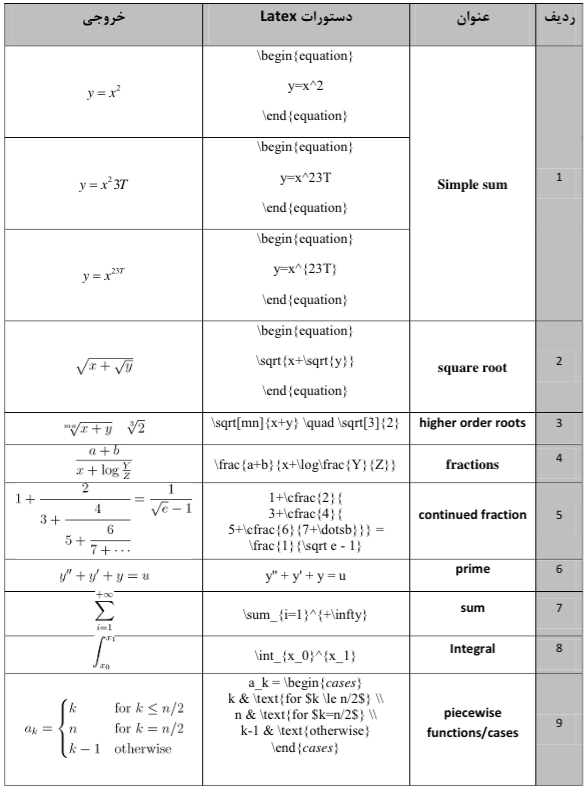
\includegraphics[width = 0.9\textwidth]{pics/math_sample_1.png}
        %     \label{LABEL_PIC_math_example}
        %     \caption{this is a pic to add here.}
        % \end{figure}
        
        \begin{figure}[hbt!]
            \centering
            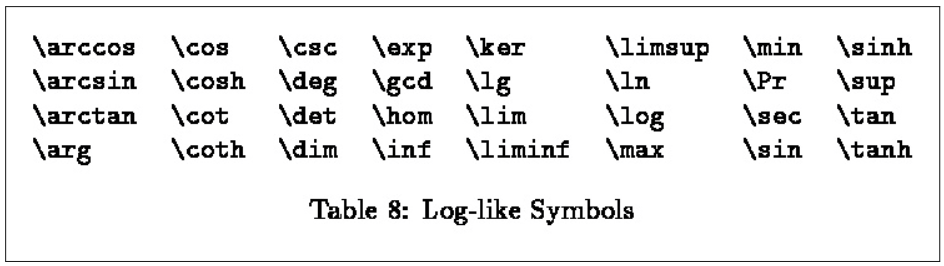
\includegraphics[width=0.5\textwidth]{pics/math_1.png}
            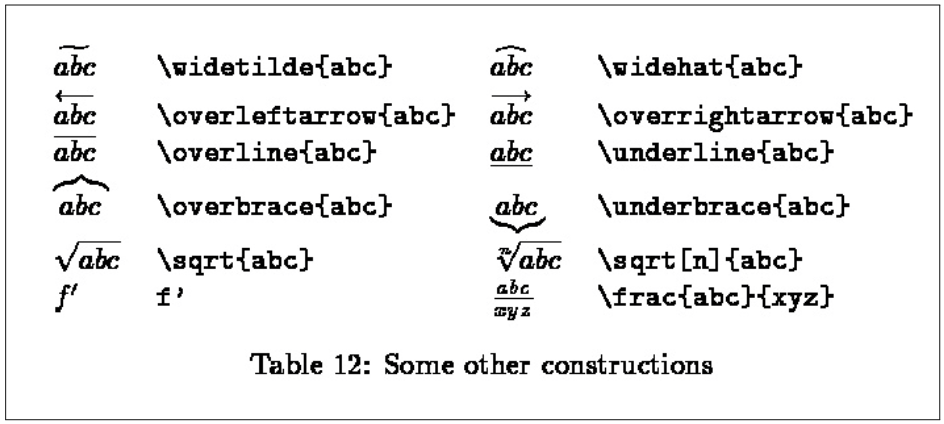
\includegraphics[width=0.5\textwidth]{pics/math_2.png}
            \caption{math formulas}
        \end{figure}

        % 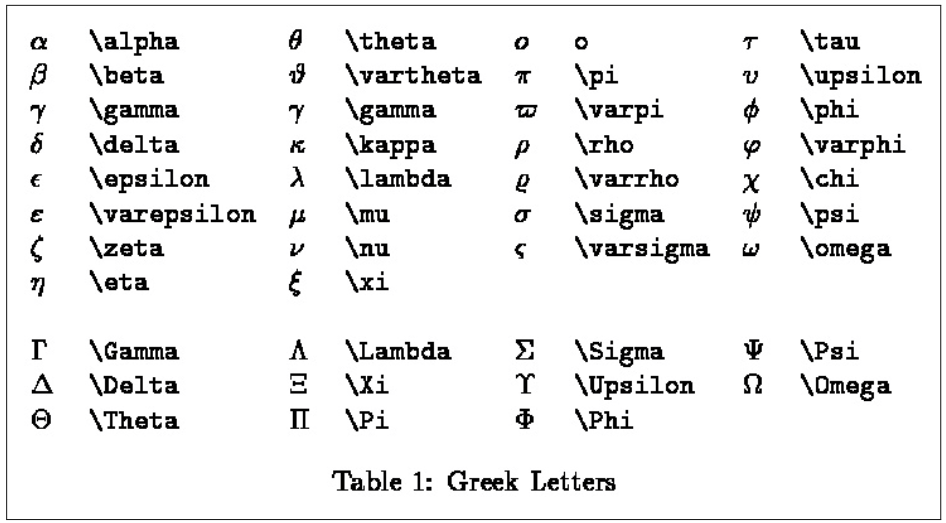
\includegraphics[width = 1\textwidth]{pics/math_alfabet.png}
        % 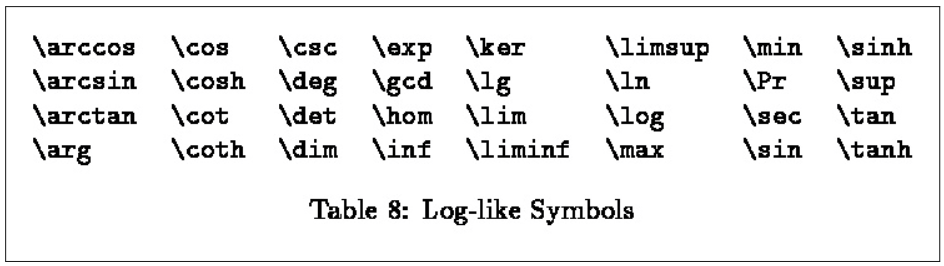
\includegraphics[width = 1\textwidth]{pics/math_1.png}
        % 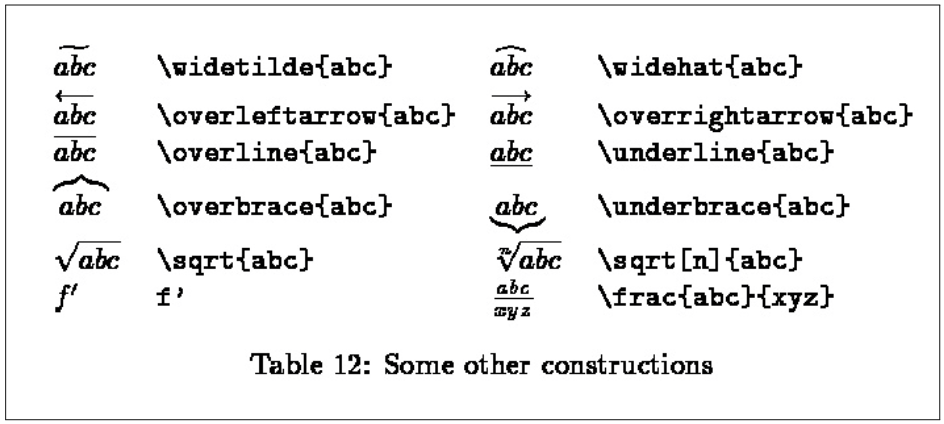
\includegraphics[width = 1\textwidth]{pics/math_2.png}
        % 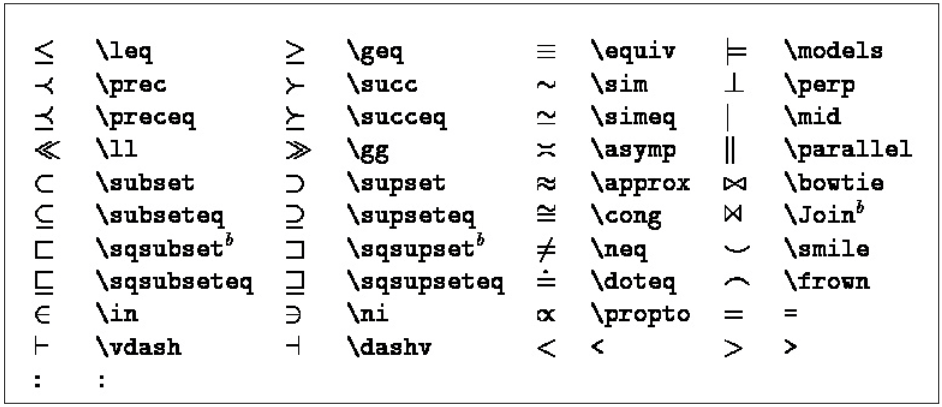
\includegraphics[width = 1\textwidth]{pics/math_3.png}
        % 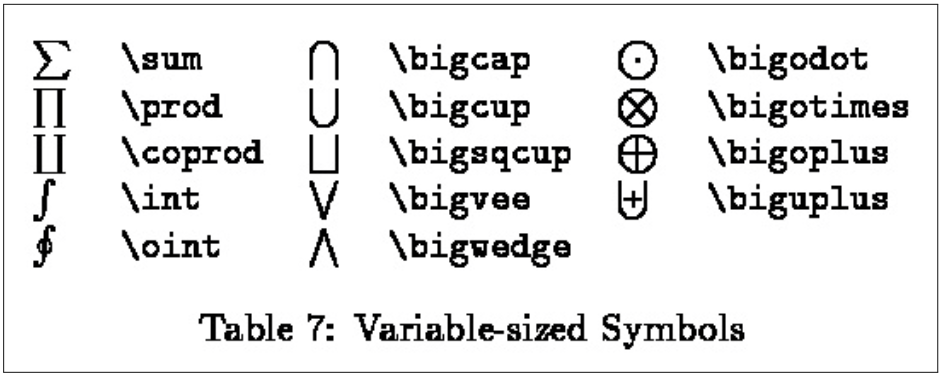
\includegraphics[width = 1\textwidth]{pics/math_4.png}
        % 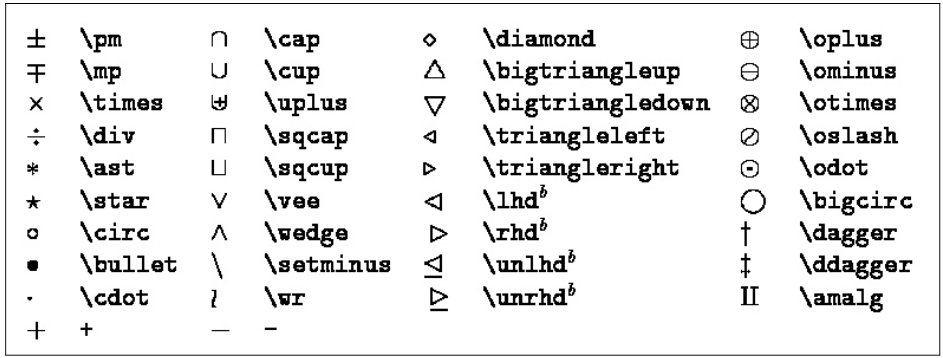
\includegraphics[width = 1\textwidth]{pics/math_5.png}
        % 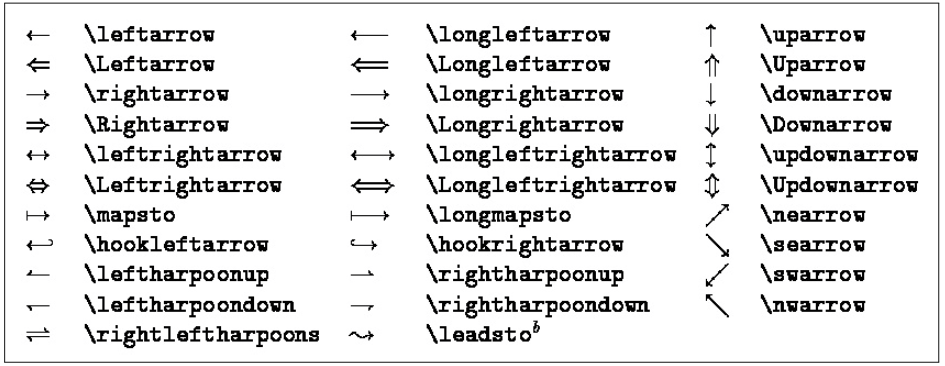
\includegraphics[width = 1\textwidth]{pics/math_6.png}

\section{References}

% \begin{frame}{Contributions}
\begin{itemize}
\item \textbf{This article uses some text from website:}
\begin{itemize}
    \setlength{\itemsep}{10pt} % Adjust the value to control the spacing
    \item \href{https://www.google.com/}{google.com}
    \item \href{https://www.akbarbaghbani.com}{akbarbaghbani.com}
\end{itemize}
\end{itemize}
% \end{frame}

\section{Bibliography}
You will probably want references in your document so that you can cite articles like \cite{Birdetal2001, soleymaniMLCourse}

\nocite{*}
\bibliographystyle{plain}
\bibliography{refs}


\section{more math}
\begin{equation}
    \iiint\limits_V f(x,y,z)\,dV = F
    \end{equation}
    
    
    \begin{equation}
    \frac{dx}{dy}=x'=\lim_{h \to 0}\frac{f(x+h)-f(x)}{h}
    \end{equation}
    
    
    \begin{equation}
    |x|=\begin{cases}
    -x, & \text{if $x < 0$}\\
    x, & \text{if $x \geq 0$} 
    \end{cases}
    \end{equation}
    
    
    \begin{equation}
    F(x)= A_0 + \sum_{n=1}^N\left[ A_n\cos{\left(\frac{2\pi nx}{P}\right)}+B_n\sin{\left(\frac{2\pi nx}{P}\right)}\right]
    \end{equation}
    
    
    \begin{equation}
    \sum_n \frac{1}{n^s}=\prod_p \frac{1}{1-\frac{1}{p^s}}
    \end{equation}
    
    
    \begin{equation*}         % equation* suppress equation numbering same for align*
    m\ddot{x}+c\dot{x}+kx=F_0\sin(2\pi ft)
    \end{equation*}
    
    
    \begin{align*}
    f(x)\quad &=\quad x^2 + 3x + 5x^2 +8 +6x\\
    &=\quad 6x^2 +9x +8\\
    &=\quad x(6x+9)+8
    \end{align*}
    
    $$
    X=\frac{F_0}{k}\frac{1}{\sqrt{(1-r^2)^2+(2\zeta r)^2}}
    $$
    
    \begin{equation}
    G_{\mu\nu} \equiv R_{\mu\nu}-\frac{1}{2}Rg_{\mu\nu}=\frac{8\pi G}{c^4}T_{\mu\nu}
    \end{equation}\\
    
    $$\mathrm{6CO_2+6H_2O \to C_6H_{12}O_6+6O_2}$$
    
    $$\mathrm{SO_4^{2-}+Ba^{2+} \to BaSO_4 }$$
    
    \begin{equation}
    \begin{pmatrix}
    a_{11}&a_{12}&\dots&a_{1n}\\
    a_{21}&a_{22}&\dots&a_{2n}\\
    \vdots&\vdots&\ddots&\vdots\\
    a_{n1}&a_{n2}&\dots&a_{nn}
    \end{pmatrix}
    \begin{pmatrix}
    v_{1}\\
    v_{2}\\
    \vdots\\
    v_{n}
    \end{pmatrix}
    =
    \begin{pmatrix}
    w_{1}\\
    w_{2}\\
    \vdots\\
    w_{n}
    \end{pmatrix}
    \end{equation}
    
    \begin{equation}
    \frac{\partial{\bf{u}}}{\partial{t}}+(\bf{u}\cdot\nabla)\bf{u}-\nu\nabla^2\bf(u)=-\nabla h
    \end{equation}
    
    \[             % This is preferred to the $$ environment 
    \alpha A \beta B \gamma \Gamma \delta \Delta \pi \Pi \omega \Omega 
    \]
    
\end{document}
